% Chapter Template

\chapter{Die 2 Modi} % Main chapter title

\label{ChapterX} % Change X to a consecutive number; for referencing this chapter elsewhere, use \ref{ChapterX}

%----------------------------------------------------------------------------------------
%	SECTION 1
%----------------------------------------------------------------------------------------

\section{Der eingebettete Modus}

Mittels Treiber lassen sich verschiedene Programmiersprachen verwenden, um Neo4j anzusteuern. Alle Klassen und Prozesse werden direkt in der Java virtual machine (JVM) ausgeführt und mittels des GraphDataBaseService  werden die benötigten Neo4j Funktionen aufgerufen und auf den Speicher angewenden. Dies wird in \ref{fig:Embedded} dargestellt.
\begin{figure}[th]
	\centering
	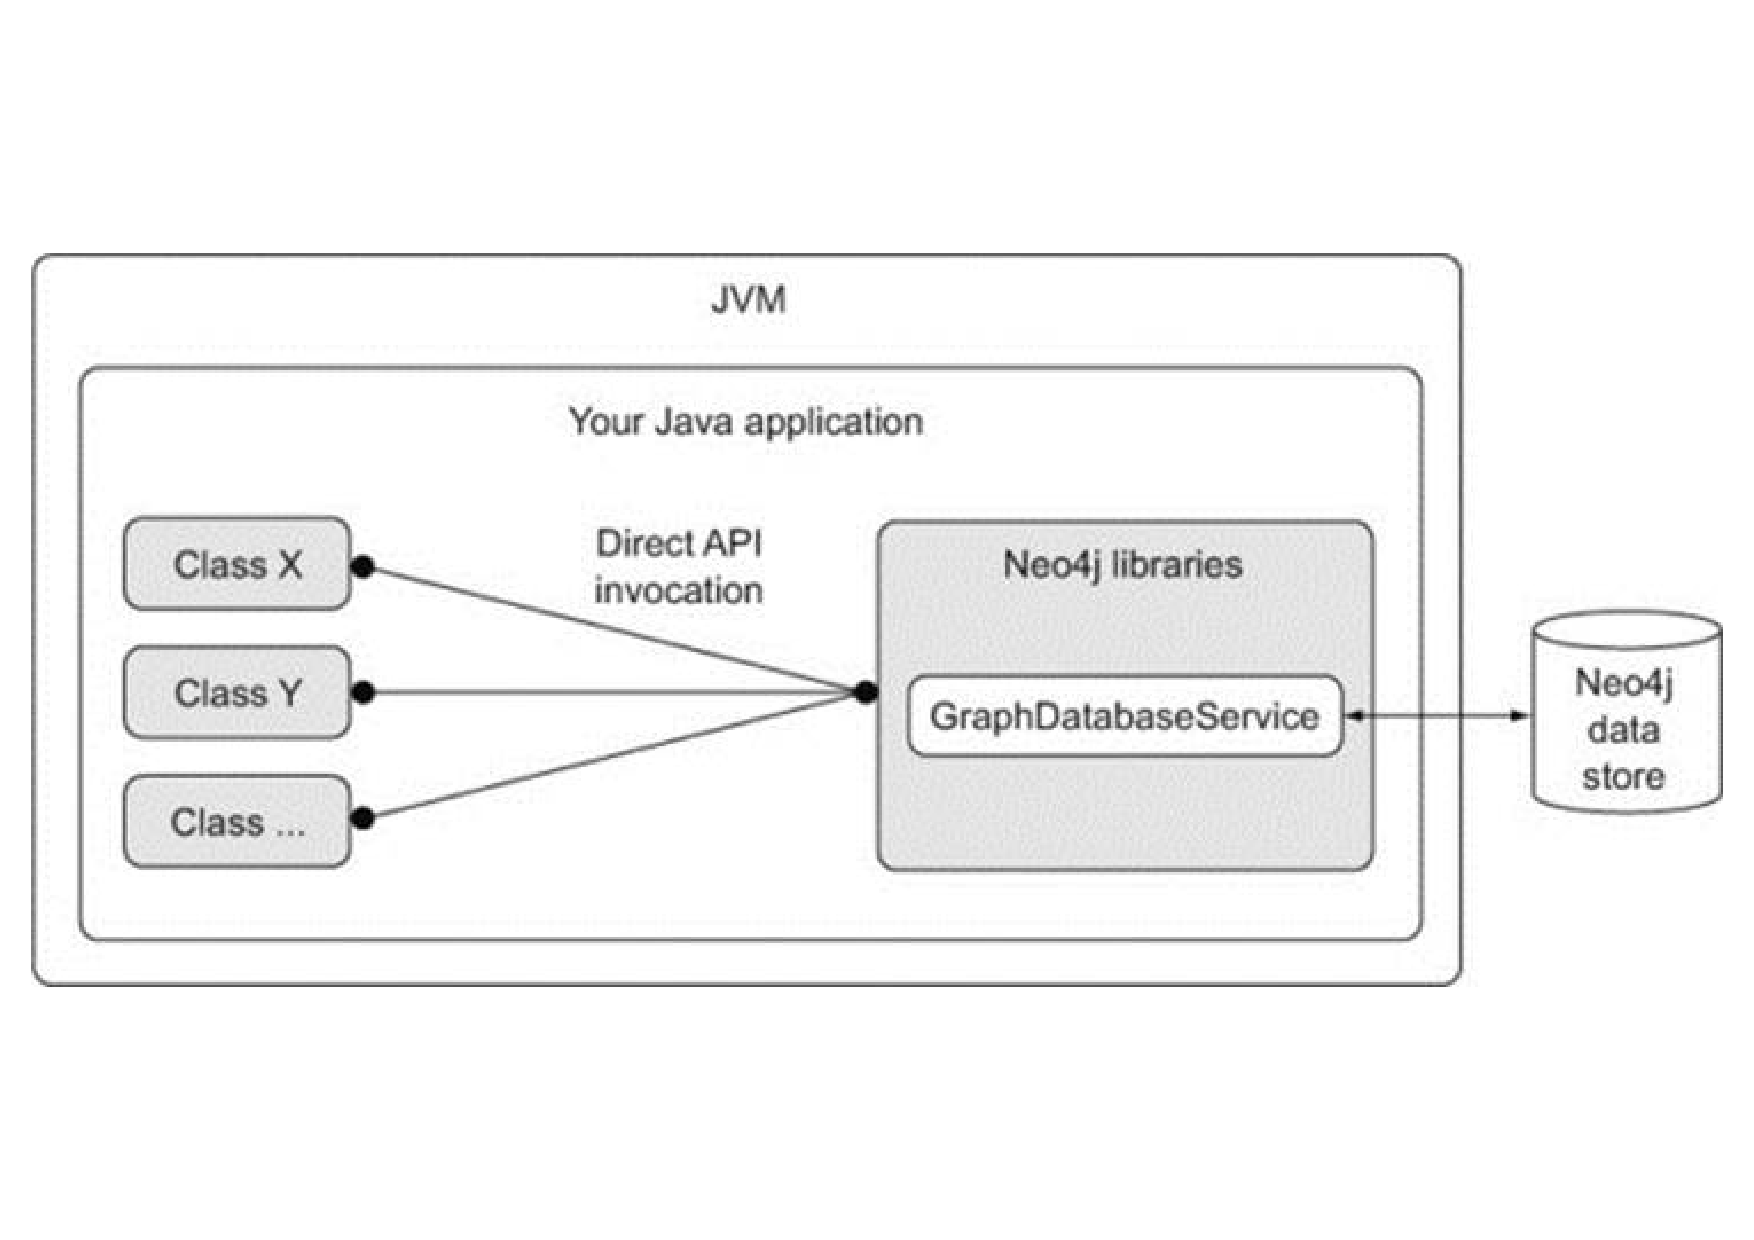
\includegraphics [width=14cm, height=12cm]{Figures/Embedded}
	\caption[Eingebettet]{Allgemeiner eingebetteteter Modus von Neo4j.}
	\label{fig:Embedded}
\end{figure}


\section{Der Server Modus}

In diesem Modus bilden die Klassen und Operationen einen eigenen Prozess und sind isoliert von der Anwendung. Die Kommunikation zwischen der Anwendung des Nutzers und der JVM findet durch die REST API[17] statt[16] und wird mittels HTTP (Hypertext Transfer Protocol) übertragen.Dies wird in \ref{fig:Embedded} verdeutlicht.
\begin{figure}[th]
	\centering
	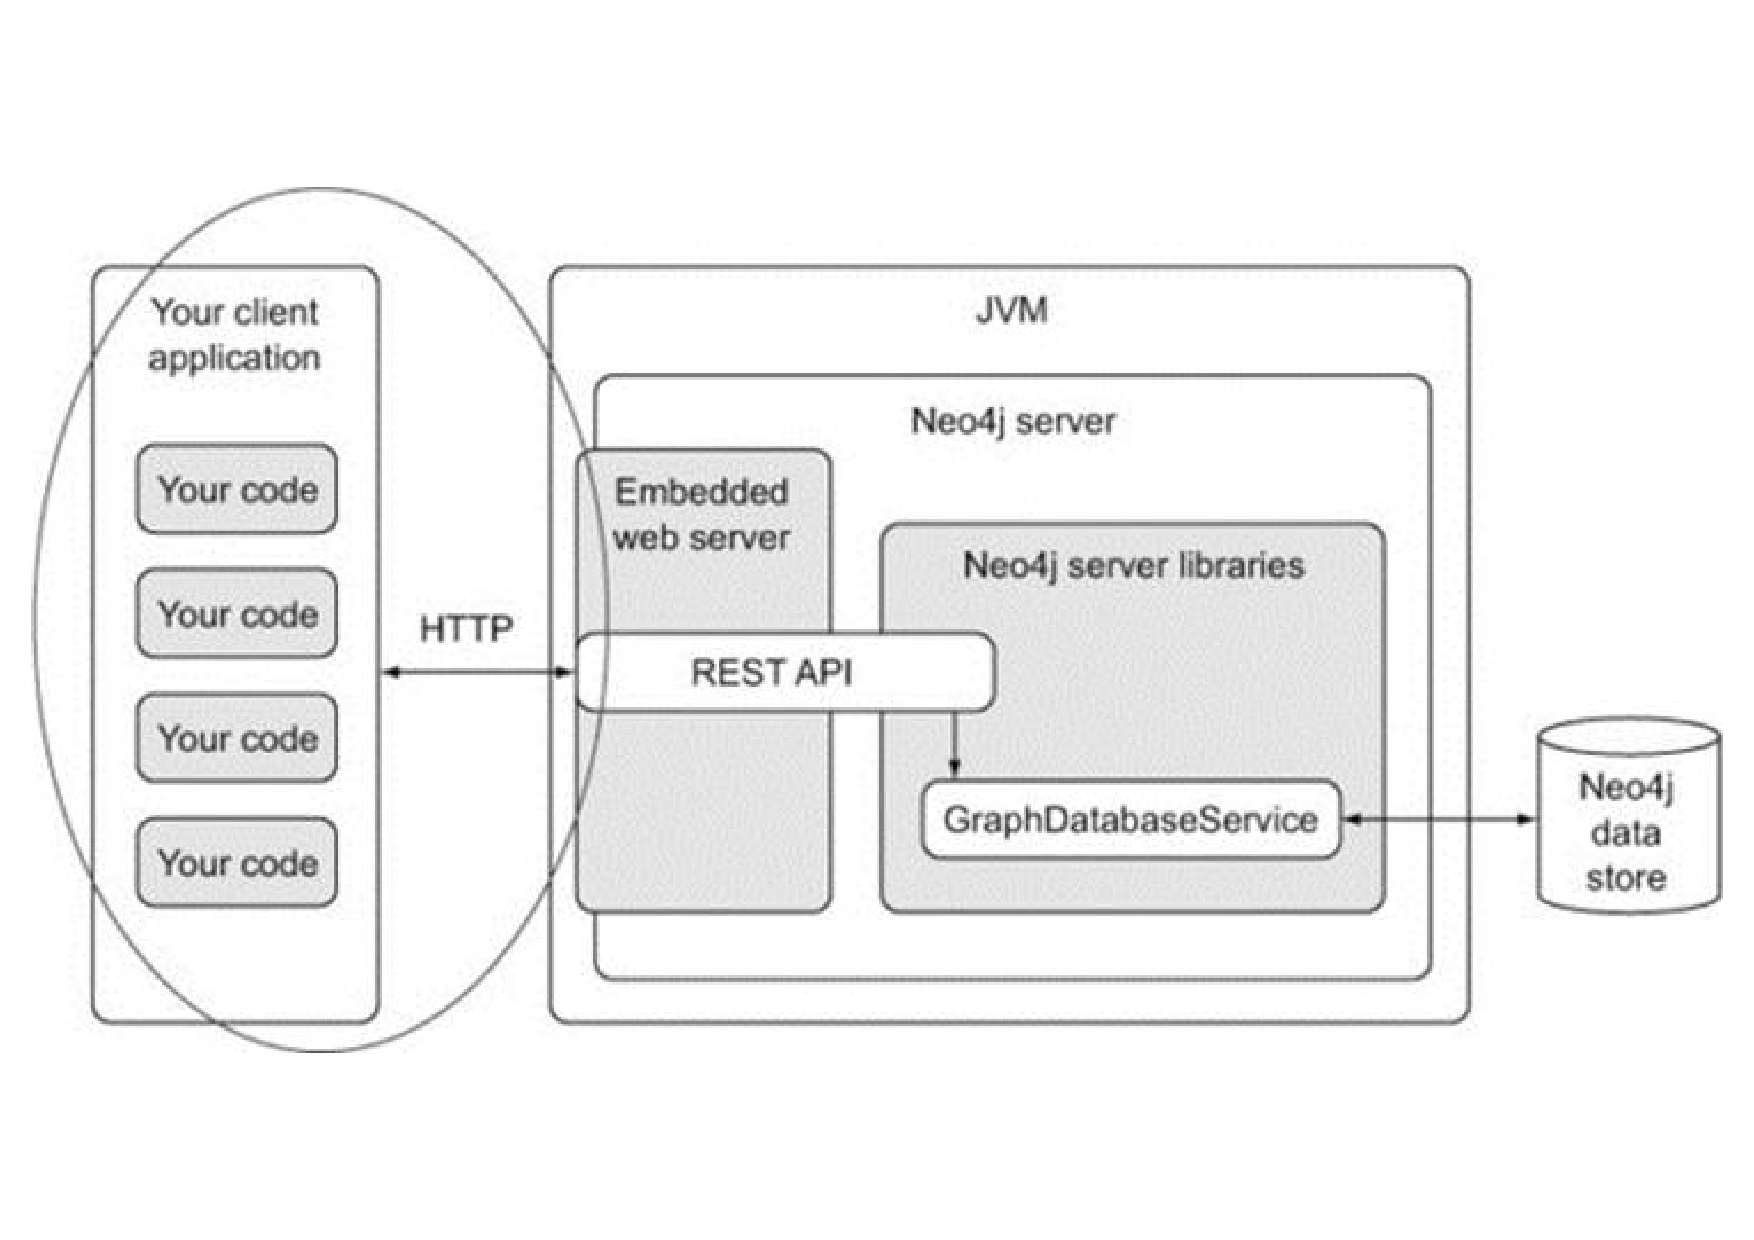
\includegraphics [width=14cm, height=12cm]{Figures/Server}
	\caption[Server]{Allgemeiner Servermodus von Neo4j.}
	\label{fig:Embedded}
\end{figure}